\documentclass{article}
\usepackage[utf8]{inputenc}
\usepackage{xurl}
\usepackage[czech]{babel}
\usepackage{csquotes}
\usepackage{dcolumn}
\usepackage{subfig}
\usepackage{graphicx}

\MakeOuterQuote{"}

\title{Metody analýzy dat I - analýza datasetu}
\author{Filip Peterek, PET0342}
\date{28. prosinec 2021}

\begin{document}

\maketitle

\section{Popis datové sady}

Datová sada obsahuje seznam nahlášených zločinů za rok 2018 ve městě Austin
v americkém státě Texas. Data byla sbírána policií města Austin a následně
veřejně publikována \cite{dataset-source}. Datová sada obsahuje 37156 záznamů
odpovídajících 37156 nahlášeným zločinům.

\subsection{Atributy datové sady}

V datové sadě se objevuje 13 atributů, které jsou popsány v tabulce \ref{tab:attributes}.

\begin{table}
  \centering
  \caption{Popis atributů datové sady}
  \label{tab:attributes}
  \makebox[\textwidth][c]{
    \begin{tabular}{ |l|l|l|l|l| }
      \hline
      Název & Popis & Typ & Datový typ & Povinný \\
      GO Primary Key & ID incidentu & numerický & celé číslo & ano \\
      Council District & městská čtvrť & kategoriální & celé číslo & ne \\
      GO Highest Offense & zločin & kategoriální & řetězec & ano \\
      Crime Type & typ zločinu & kategoriální & řetězec & ano \\
      GO Report Date & den nahlášení & numerický & datum & ano \\
      GO Location & místo odehrání zločinu & kategoriální & řetězec & ne \\
      GO X Coordinate & místo odehrání zločinu & numerický & desetinné číslo & ne \\
      GO Y Coordinate & místo odehrání zločinu & numerický & desetinné číslo & ne \\
      Clearance Status & stav policejního pátrání & kategoriální & řetězec & ne \\
      Clearance Date & datum vyřešení případu & numerický & datum & ne \\
      GO District & policejní sektor & kategoriální & řetězec & ano \\
      GO Location Zip & poštovní směrovací číslo & kategoriální & celé číslo & ne \\
      GO Census Tract & čtvrť podle počtu obyvatel & kategoriální & desetinné číslo & ne \\
      \hline
    \end{tabular}
  }
\end{table}

\section{Výsledky analýzy}

\subsection{Počty zločinů}

Počty jednotlivých zločinů, viz graf \ref{fig:crime_counts}, jistě nijak zarážející nejsou. Naprosto
převažují krádeže, v tomto případě se z velké části s vysokou pravděpodobností jedná převážně o kapsářství
a podobné drobné krádeže. Počet vloupání do domu je v porovnání s drobnějšími, méně závažnými kráděžemi méně
než pětinový. Násilné činy tak časté nejsou, přesto se jich několik objevuje.

\begin{figure}
  \centering
  \makebox[\textwidth][c]{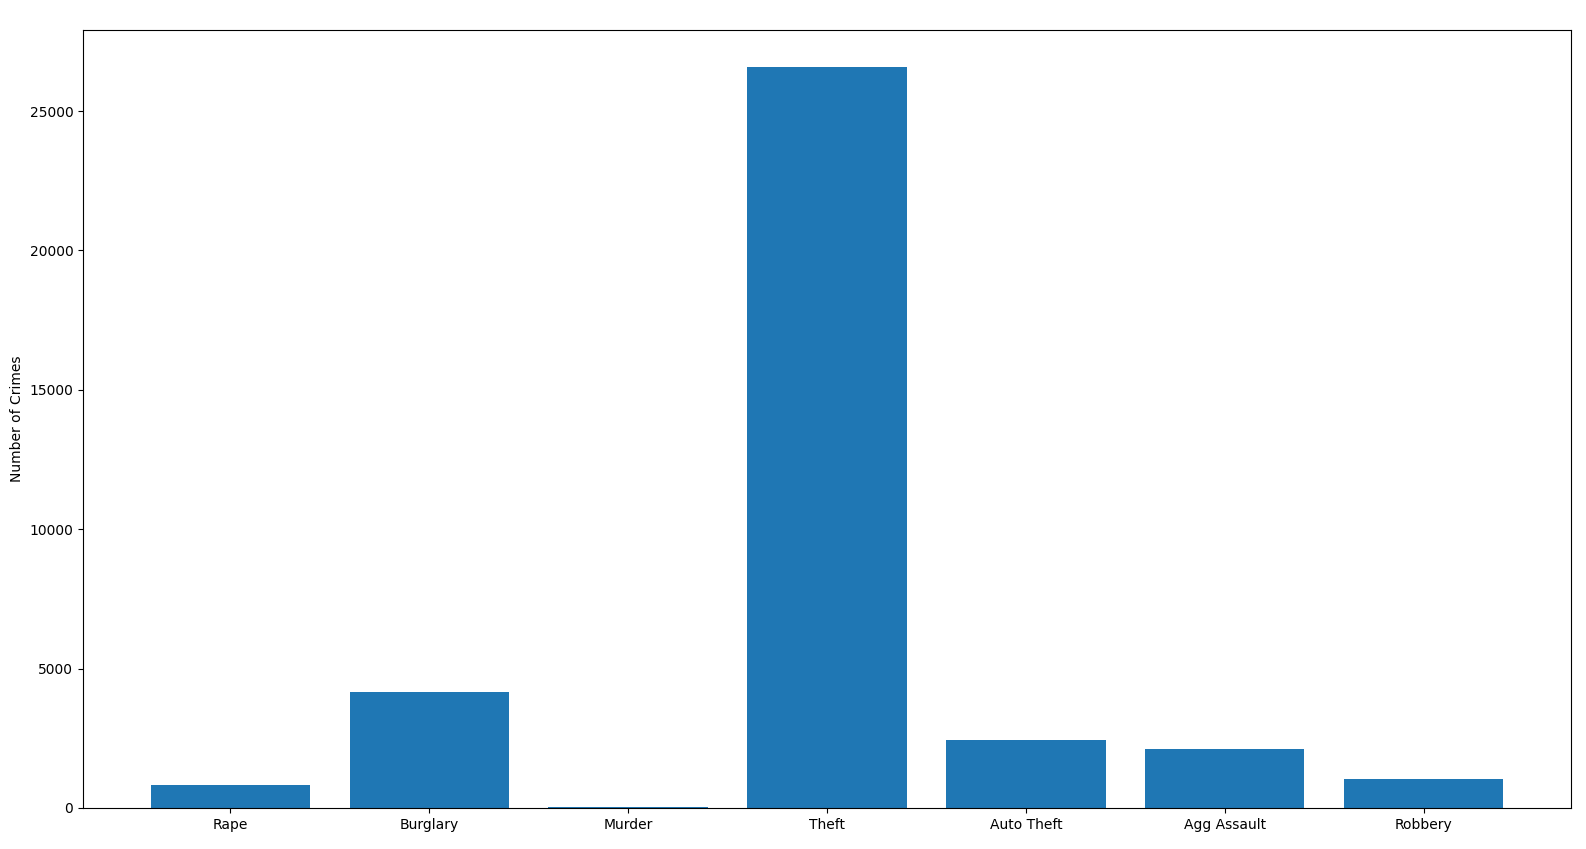
\includegraphics[width=1.6\textwidth]{figures/crime_counts.png}}
  \caption{Počet nahlášených zločinů podle kategorie}
  \label{fig:crime_counts}
\end{figure}

Velmi znepokojující jsou počty nahlášeného násilí na dětech (graf \ref{fig:crime_against_children}).
Austin je velké město, a proto se s vysokou pravděpodobností objeví zločiny všech možných typů,
přesto řádově stovky případů zneužívání dětí je alarmující číslo.

\begin{figure}
  \centering
  \makebox[\textwidth][c]{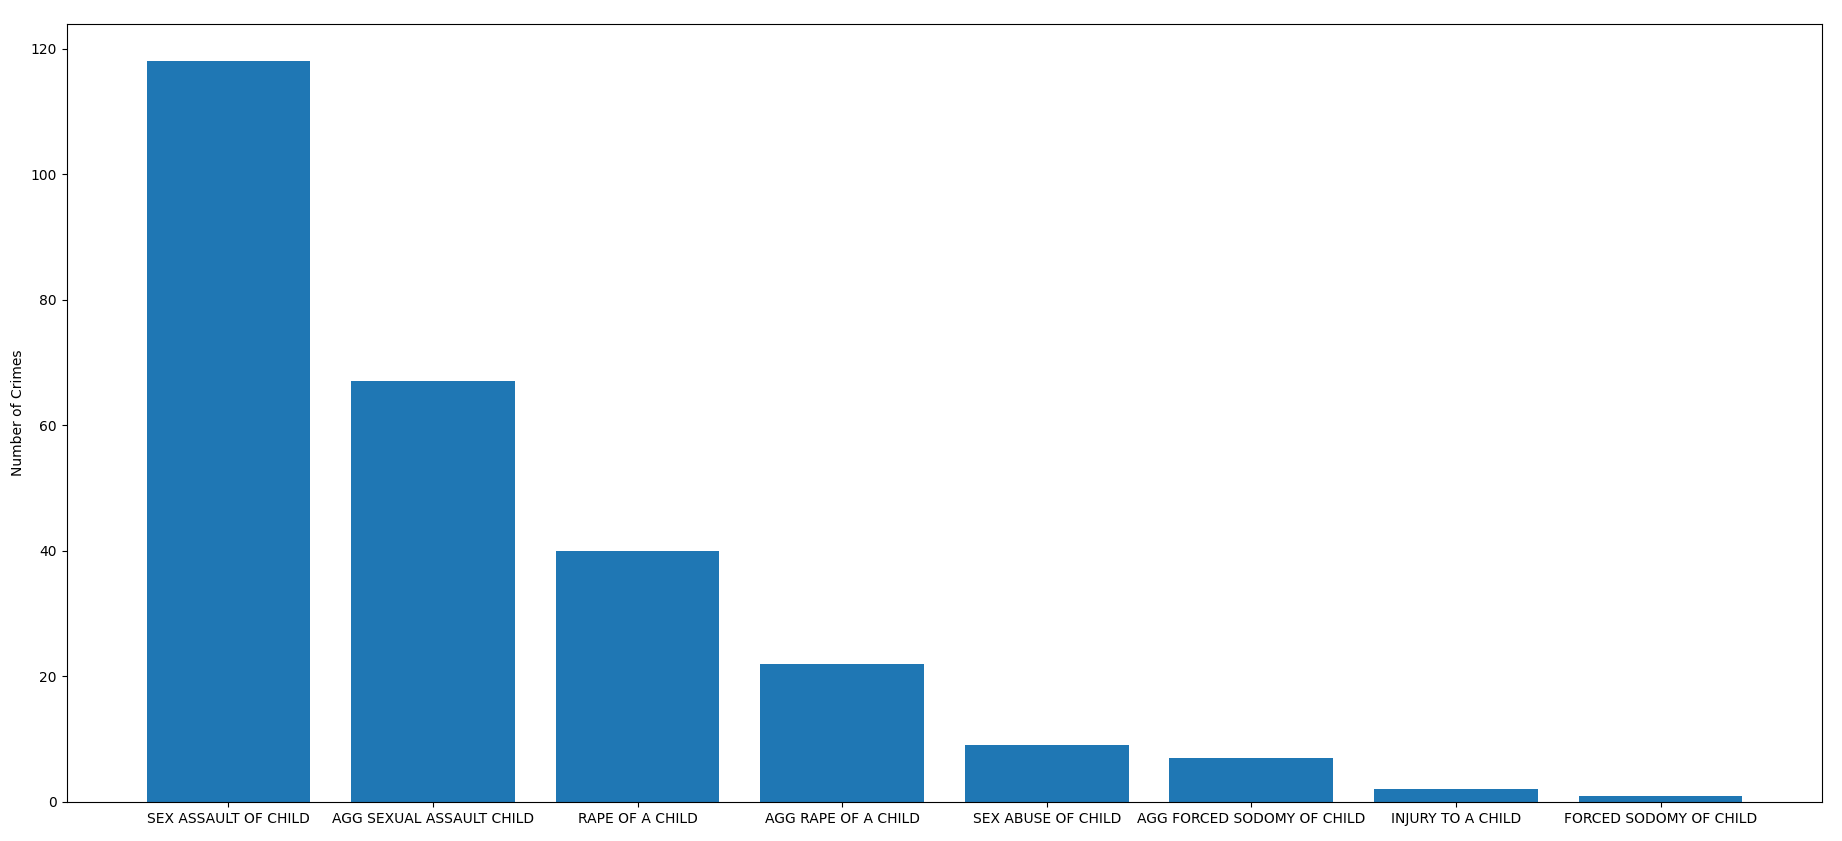
\includegraphics[width=1.6\textwidth]{figures/crime_against_children.png}}
  \caption{Počet nahlášených zločinů proti dětem}
  \label{fig:crime_against_children}
\end{figure}

Počet nahlášených zločinů podle kalendářního měsíce (graf \ref{fig:crime_per_each_month}) není
nijak zajímavý. Nejméně zločinů bylo nahlášeno v únoru -- nepřekvapivě, neboť se jedná
o nejkratší měsíc v roce. Nejvíce zločinů bylo nahlášeno v říjnu. Překvapivě může působit
fakt, že nedošlo k nárůstu zločinnosti v letních měsících. Austin sice nepatří mezi
nejvyhledávanější turistické destinace ve Spojených státech, přesto se však jedná o město
s bohatým kulturním vyžitím. I tak ale v létě zločinnost nestoupla.

\begin{figure}
  \centering
  \makebox[\textwidth][c]{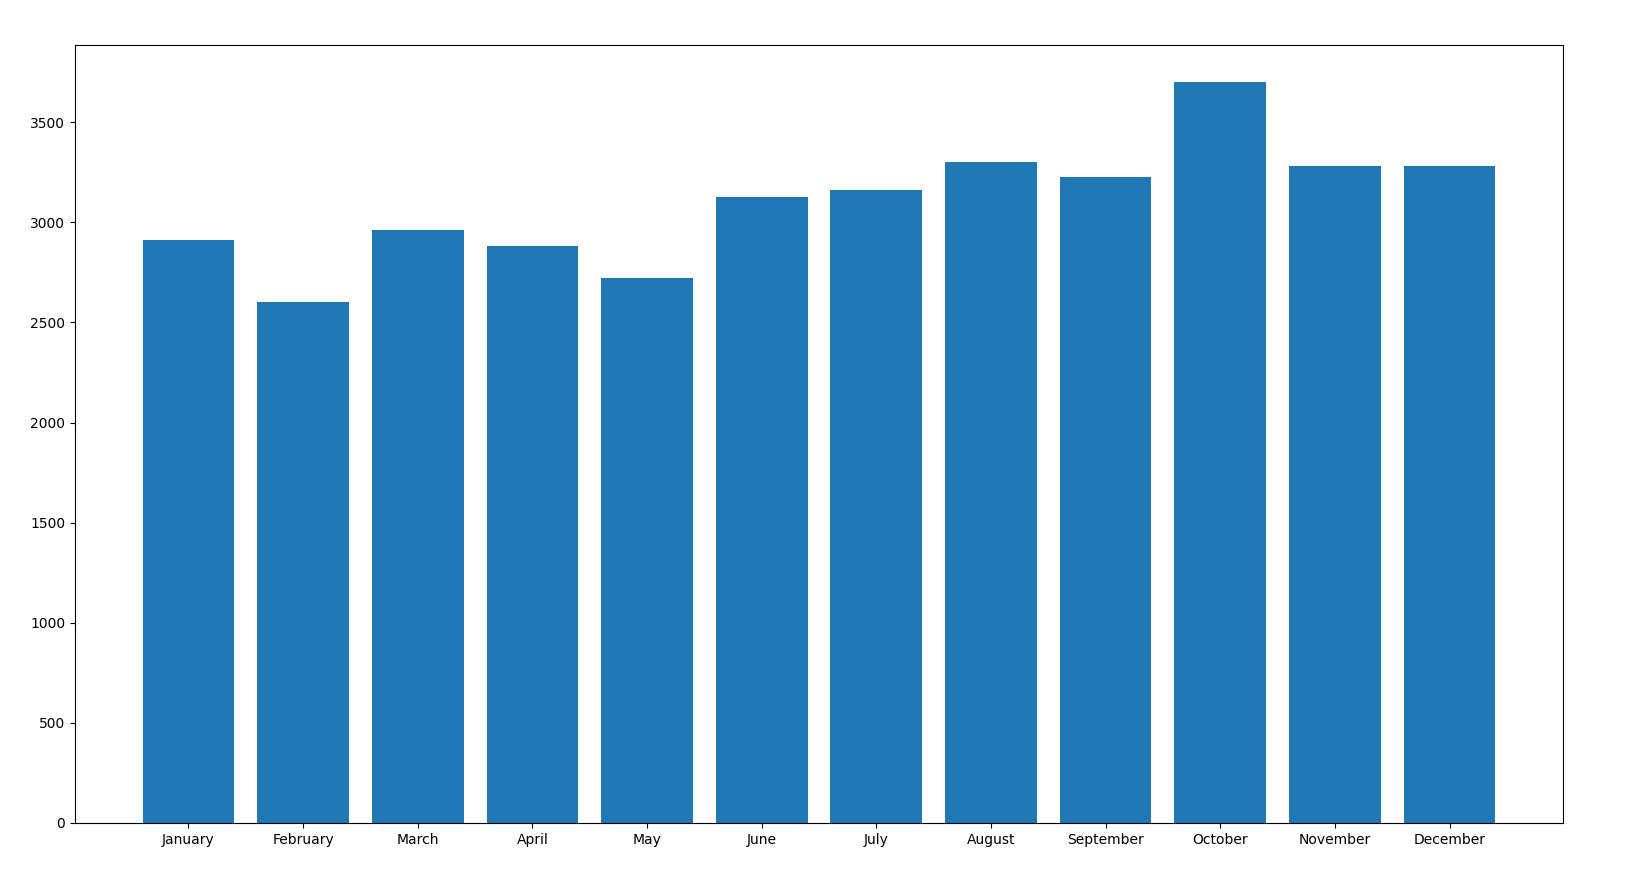
\includegraphics[width=1.6\textwidth]{figures/crime_per_each_month.png}}
  \caption{Počet nahlášených zločinů podle kalendářního měsíce}
  \label{fig:crime_per_each_month}
\end{figure}

Drobný nárůst zločinnosti v říjnu může vzbudit určitou zvědavost, při podrobnějším prozkoumání
ovšem zjistíme, že se neobjevily žádné zajímavé zločiny (např. hromadné nahlášení daňových úniků),
jednalo se převážně o drobné krádeže. Přesto tato skutečnost může být zajímavá pro policejní
oddělení města Austin.

\begin{figure}
  \centering
  \makebox[\textwidth][c]{\includegraphics[width=1.6\textwidth]{figures/october_crime.png}}
  \caption{Sedm nejčastějších zločinů v říjnu 2018}
  \label{fig:october_crime}
\end{figure}

\subsection{Řešení zločinů}

Vzorného občana určitě znepokojí množství nevyřešených případů. Z grafu \ref{fig:clearance_status}
lze vyčíst, že naprostá většina případů zůstává nevyřešena.

\begin{figure}
  \centering
  \makebox[\textwidth][c]{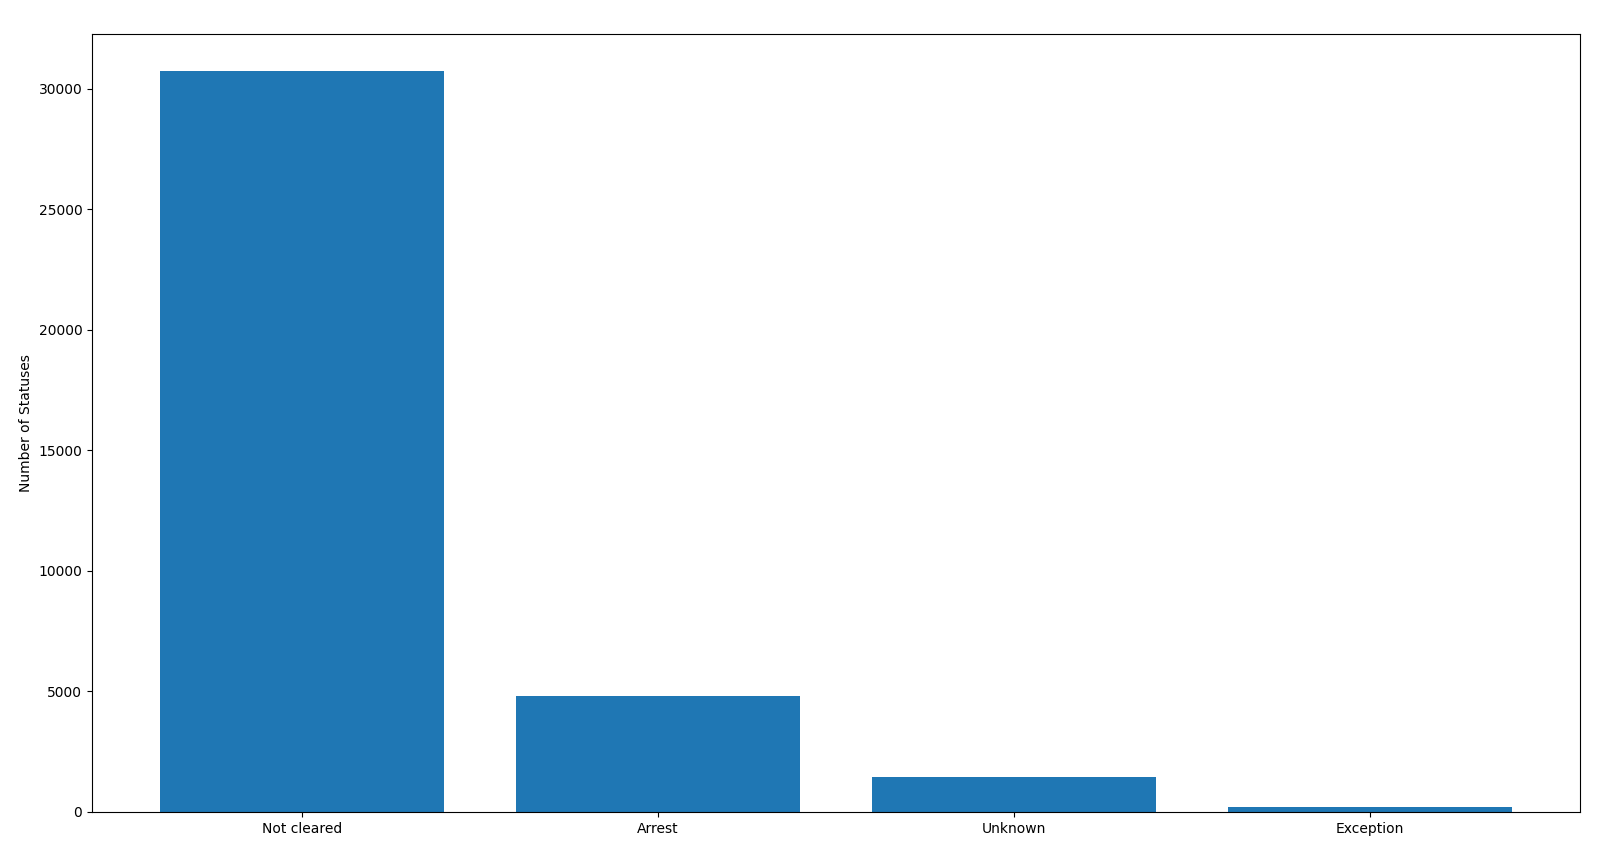
\includegraphics[width=1.6\textwidth]{figures/clearance_status.png}}
  \caption{Četnosti statusů policejního pátrání}
  \label{fig:clearance_status}
\end{figure}

Z grafu průměrné délky řešení případu (graf \ref{fig:clearance_time}) zjistíme, že nejkratší dobu trvá
řešení krádeží. Graf znázorňuje pouze úspěšně vyřešené případy. Nejrychleji jsou v průměru řešeny
krádeže. Nejdéle jsou řešeny případy znásilnění, jejichž řešení trvá v průměru přes 80 dní.
Možná překvapivě jsou případy vražd a zabití vyřešeny v průměru do jednoho měsíce.

\begin{figure}
  \centering
  \makebox[\textwidth][c]{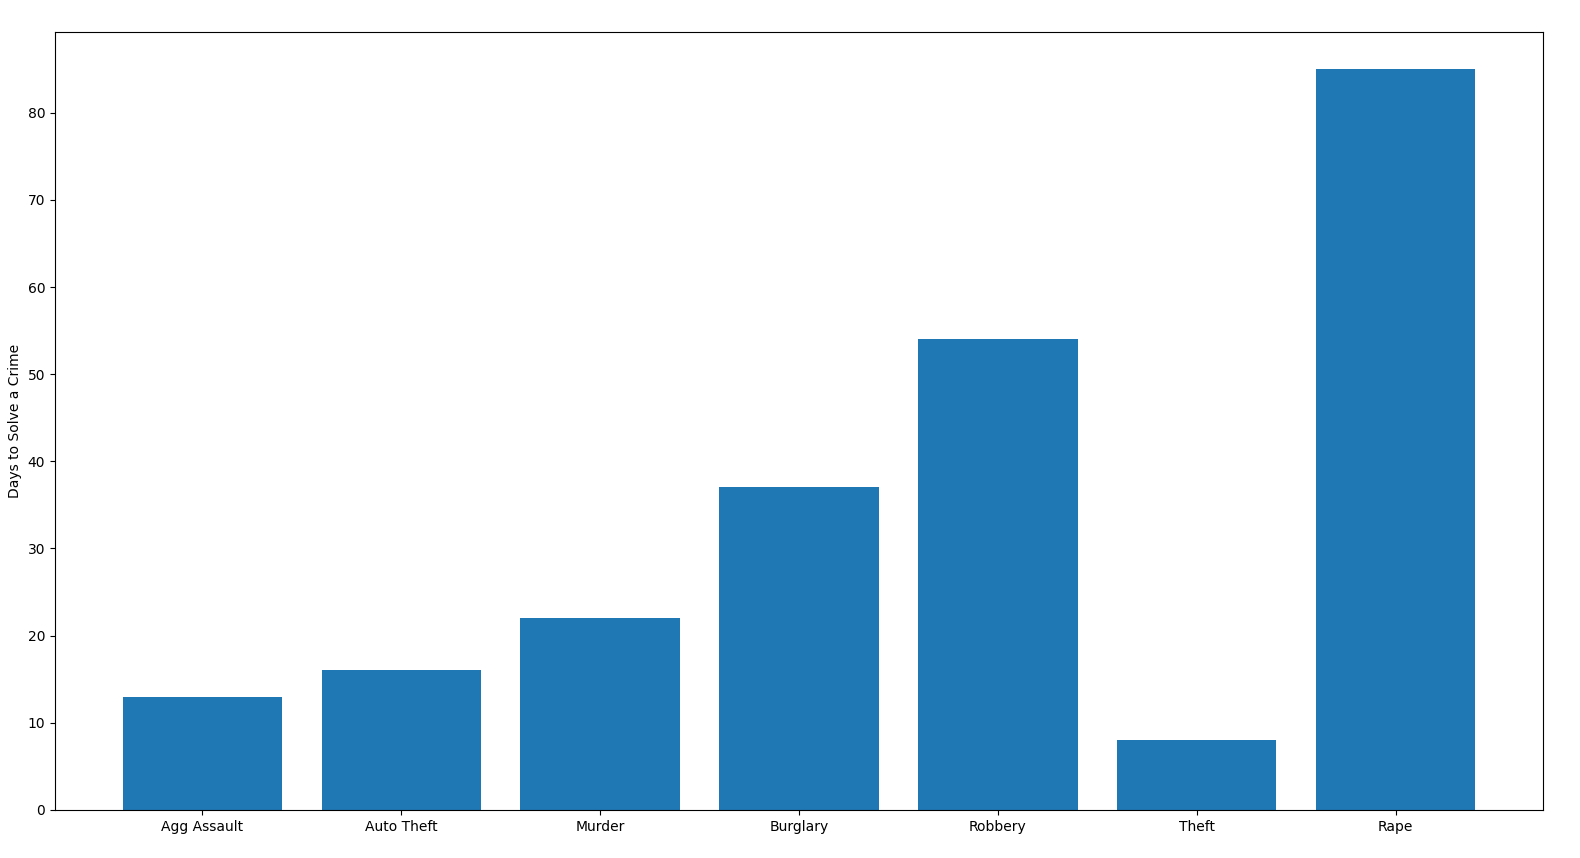
\includegraphics[width=1.6\textwidth]{figures/clearance_time.png}}
  \caption{Průměrná doba úspěšného řešení}
  \label{fig:clearance_time}
\end{figure}

Pokud se podíváme na pět nejdéle řešených případů (graf \ref{fig:top_clearance_times}), zjistíme, že byly
všechny řešeny déle než rok. Jinak ale nezjistíme žádný zajímavější trend, mezi nejdéle řešenými
případy najdeme různé typy zločinů. Překvapivě působí pouze fakt, že jsou délky řešení jednotlivých 
případů daleko za průměrem úspěšného řešení konkrétního typu zločinu.

Ovšem podíváme-li se na průměrnou délku řešení případu, medián délky, a varianci (graf
\ref{tab:avg_clearance}) (včetně uzavření nevyřešených případů), zjistíme, že průměr (a ani medián),
nejsou příliš vypovídající.

\begin{table}
  \centering
  \caption{Délka řešení případu}
  \label{tab:avg_clearance}
  \begin{tabular}{ |l|l| }
  \hline
      Průměr & 16.0 \\
      Medián & 8.0 \\
      Variance & 1172 \\
  \hline
  \end{tabular}
\end{table}

\begin{figure}
  \centering
  \makebox[\textwidth][c]{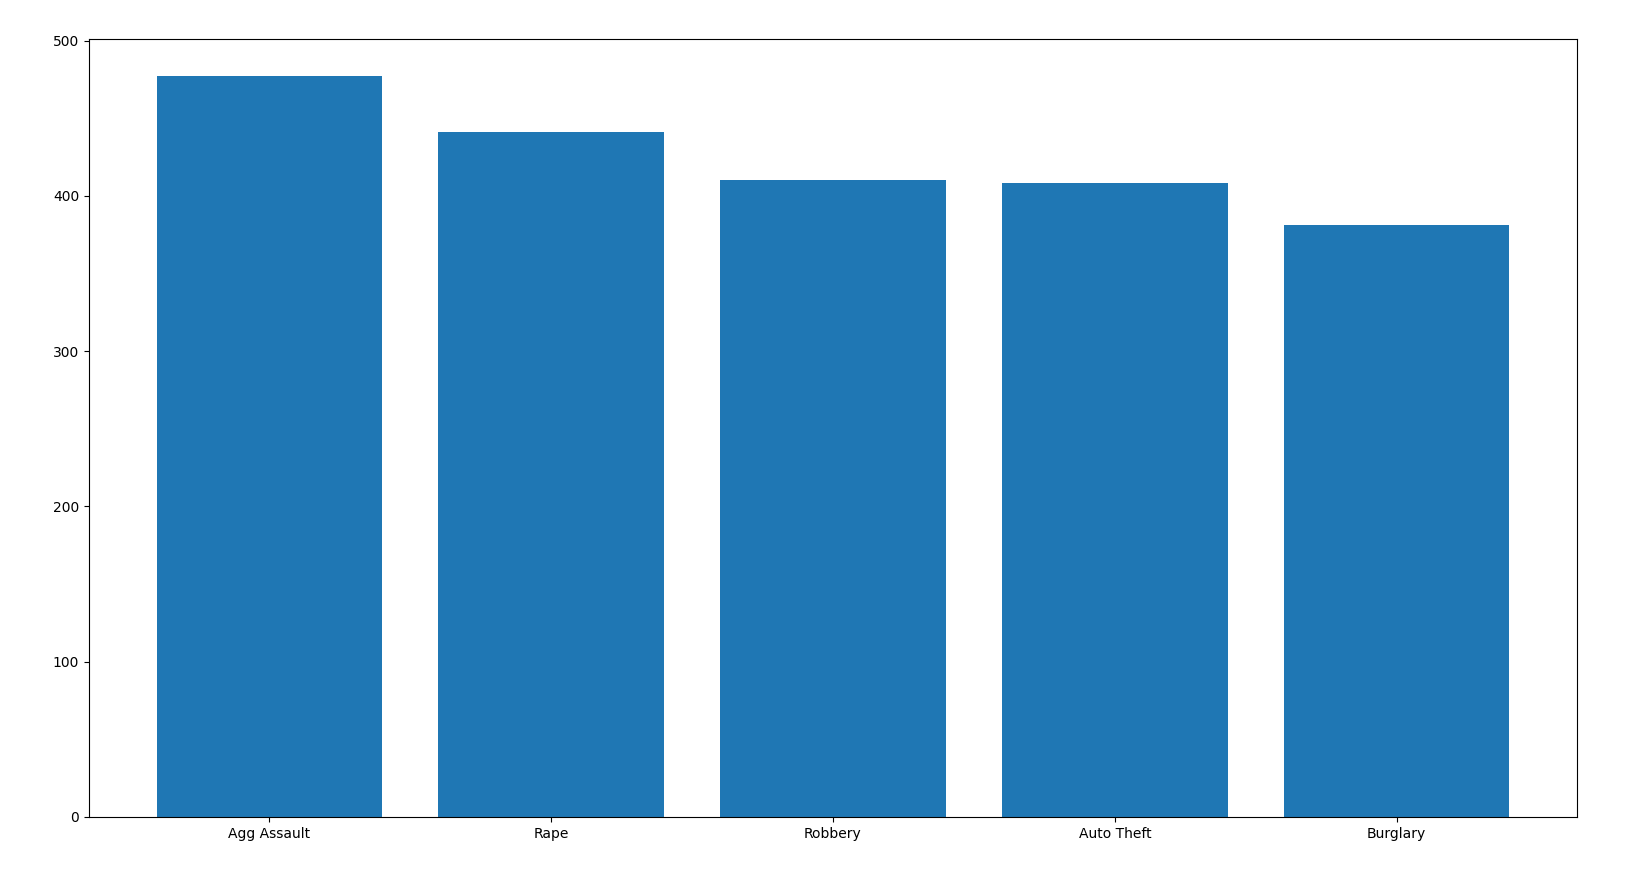
\includegraphics[width=1.6\textwidth]{figures/top_clearance_times.png}}
  \caption{Nejdéle řešené jednotlivé případy}
  \label{fig:top_clearance_times}
\end{figure}

Počty uzavřených případů seskupených podle kalendářního měsíce (graf \ref{fig:clearance_by_month}) převážně
kopírují počty nahlášených případů. Nejvíce případů bylo uzavřeno v říjnu a listopadu, což pouze reflektuje
fakt, že bylo v říjnu nahlášeno nejvíce případů -- z velké části se jednalo převážně o drobné krádeže,
které jsou zpravidla uzavírány velmi rychle. Nejméně případů bylo vyřešeno v únoru. Tato informace
je také nepřekvapivá, jelikož se jedná o nejkratší měsíc v roce.

\begin{figure}
  \centering
  \makebox[\textwidth][c]{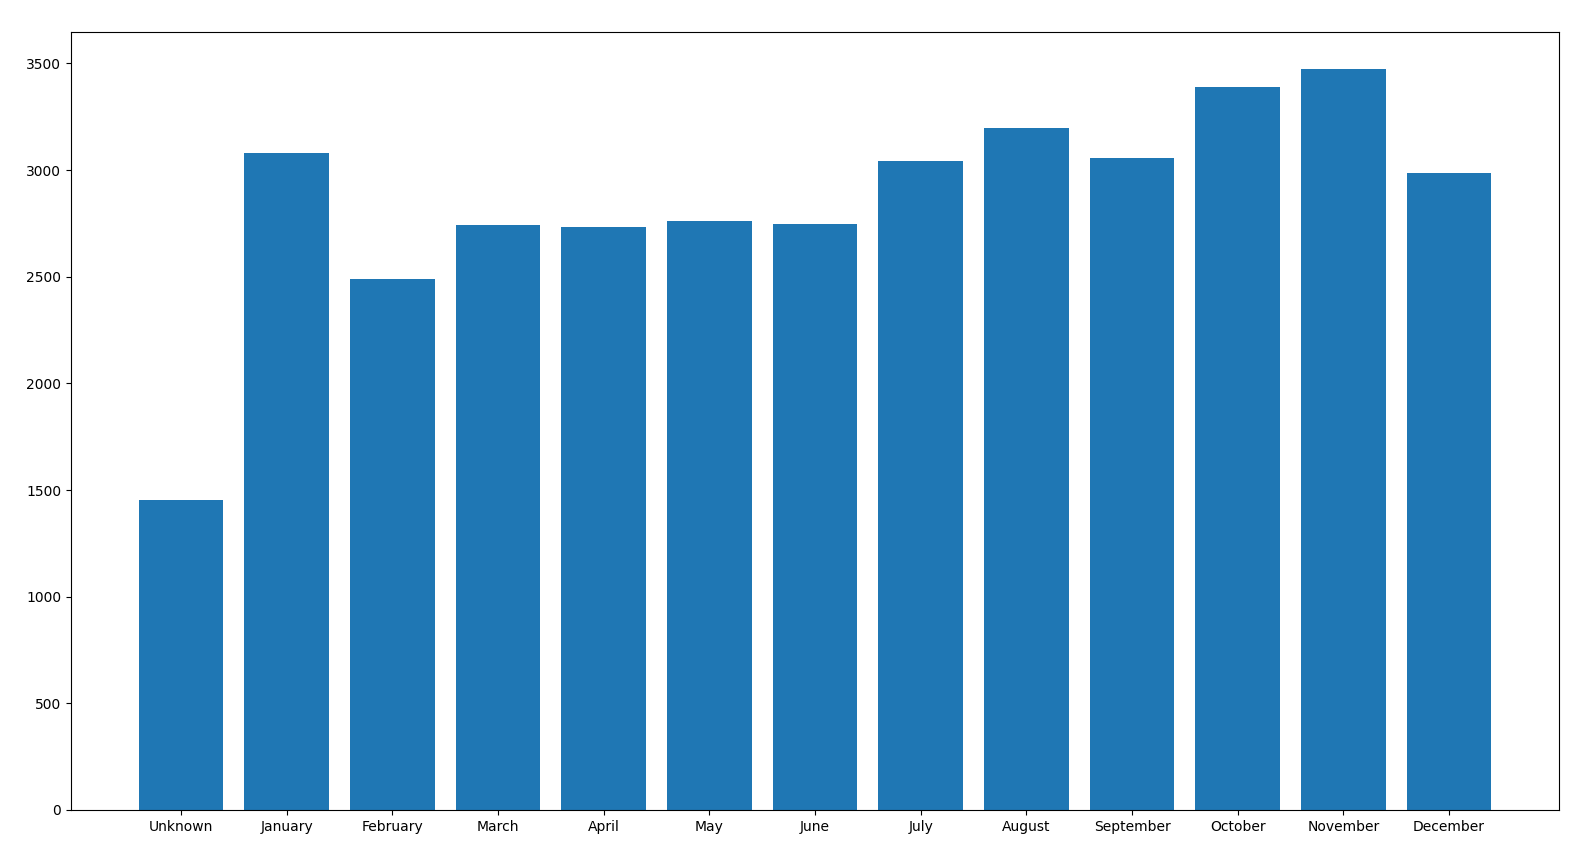
\includegraphics[width=1.6\textwidth]{figures/clearance_by_month.png}}
  \caption{Počet uzavřených případů podle kalendářního měsíce}
  \label{fig:clearance_by_month}
\end{figure}

Děsivě může působit poměr vyřešených případů v poměru k celkovému počtu případů (graf
\ref{fig:solved_percentage}). Méně než pětina vloupání, přibližně pětina krádeží aut, a přibližně
čtvrtina znásilnění skončila úspěšným vyřešením případu (zatčením pachatele nebo výjimečným řešením).
Statistika násilných napadení je poněkud lepší, více než polovina případů skončila úspěšným vyřešením.
Nejlepší statistiku nalezneme u zabití (ať už úmyslných nebo neúmyslných). 27 z celkového počtu 32 případů zabití,
tedy přes 80 \%, skončilo nalezením pachatele. Z grafu tedy vyplývá, že trváte-li nutně na dopadení
pachatele, musíte se nechat zavraždit.

\begin{figure}
  \centering
  \makebox[\textwidth][c]{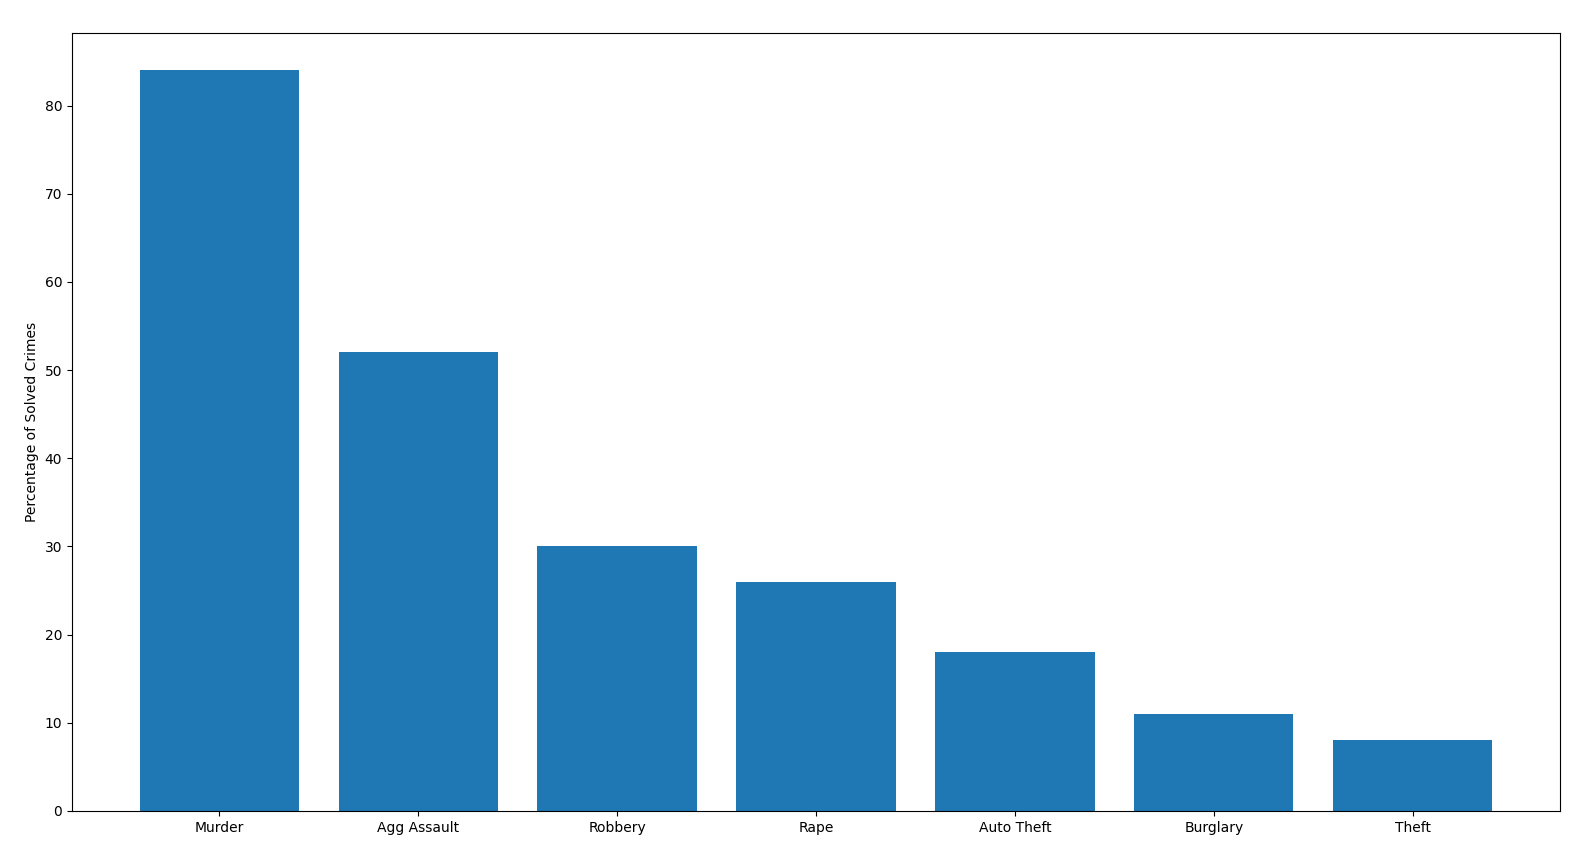
\includegraphics[width=1.6\textwidth]{figures/solved_percentage.png}}
  \caption{Poměr úspěšně vyřešených případů (v procentech)}
  \label{fig:solved_percentage}
\end{figure}

\subsection{Bezpečnost městských částí}

Případného návštěvníka či obyvatele texaského města Austin může zajímat statistika nejméně
bezpečných ulic (graf \ref{fig:worst_streets}). Při bližším prozkoumání však zjistíme, že ty nejméně
bezpečné ulice jsou zároveň jedny z nejdelších ulic v Austinu, a jedná se o ulice, které se
většinou táhnou přes polovinu města.

\begin{figure}
  \centering
  \makebox[\textwidth][c]{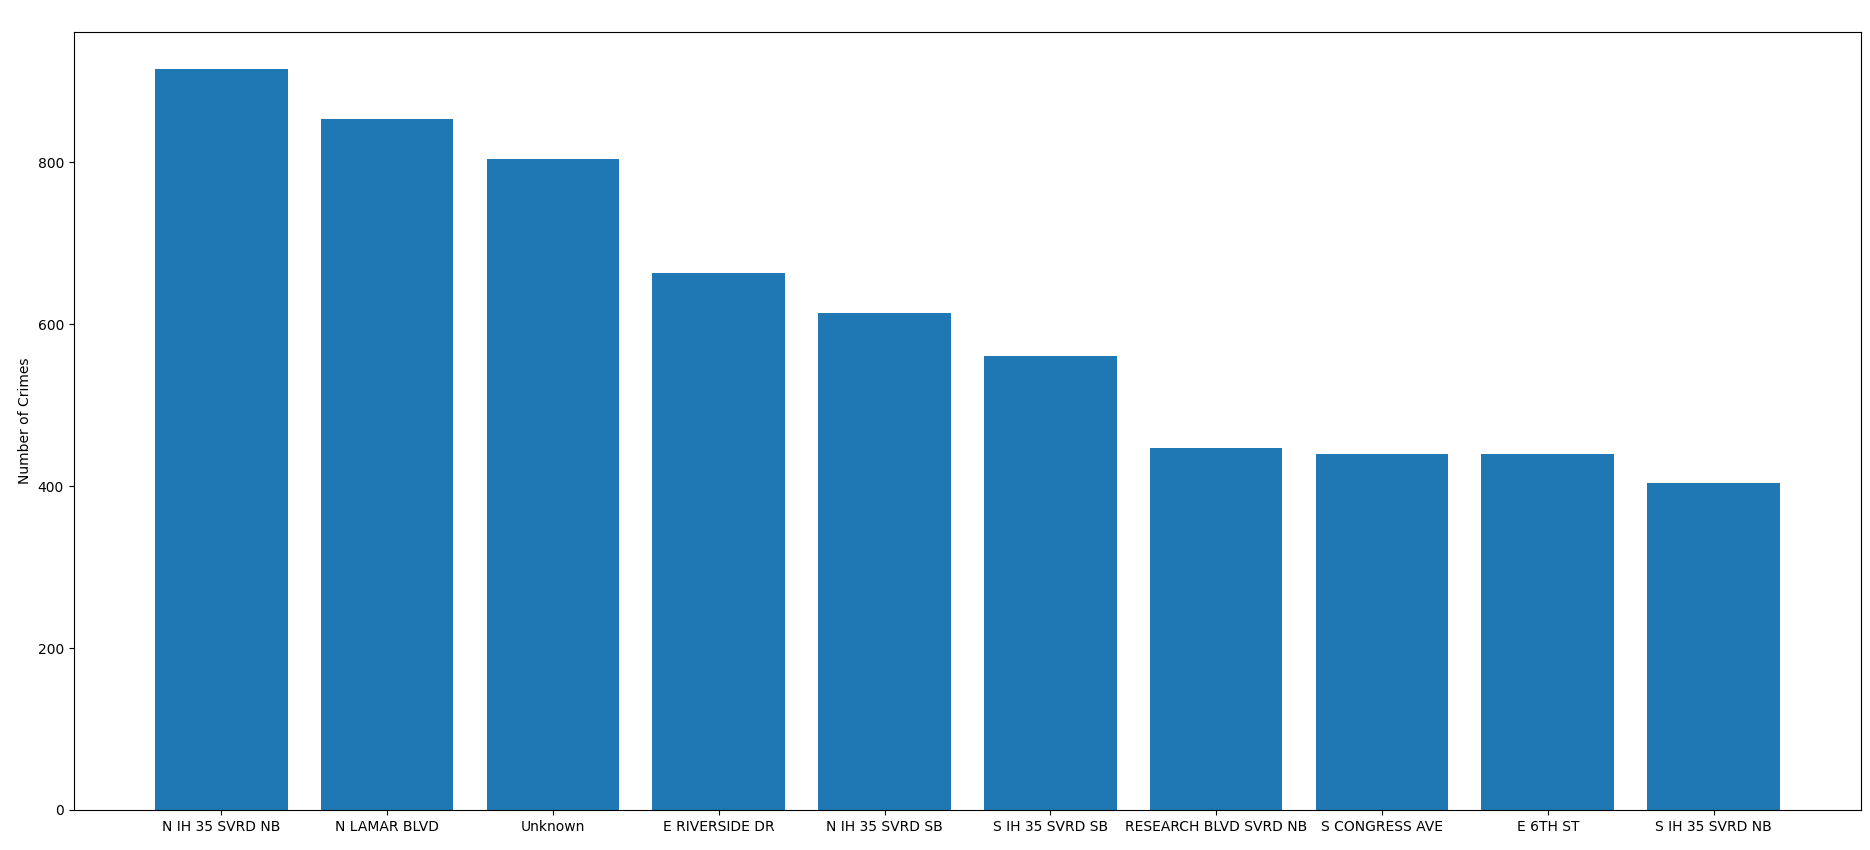
\includegraphics[width=1.6\textwidth]{figures/worst_streets.png}}
  \caption{Ulice s nejvyšším počtem nahlášených zločinů}
  \label{fig:worst_streets}
\end{figure}

Z charakteristiky datové sady vyplývá, že datová sada nebude obsahovat ulice, na kterých k žádnému
zločinu nedošlo. Mezi ulicemi, na kterých byl nahlášen alespoň jeden zločin, najdeme spoustu ulic,
kde došlo k nahlášení právě jednoho zločinu (graf \ref{fig:safest_streets}). Proto statistika nejbezpečnějších
ulic není příliš vypovídající.

\begin{figure}
  \centering
  \makebox[\textwidth][c]{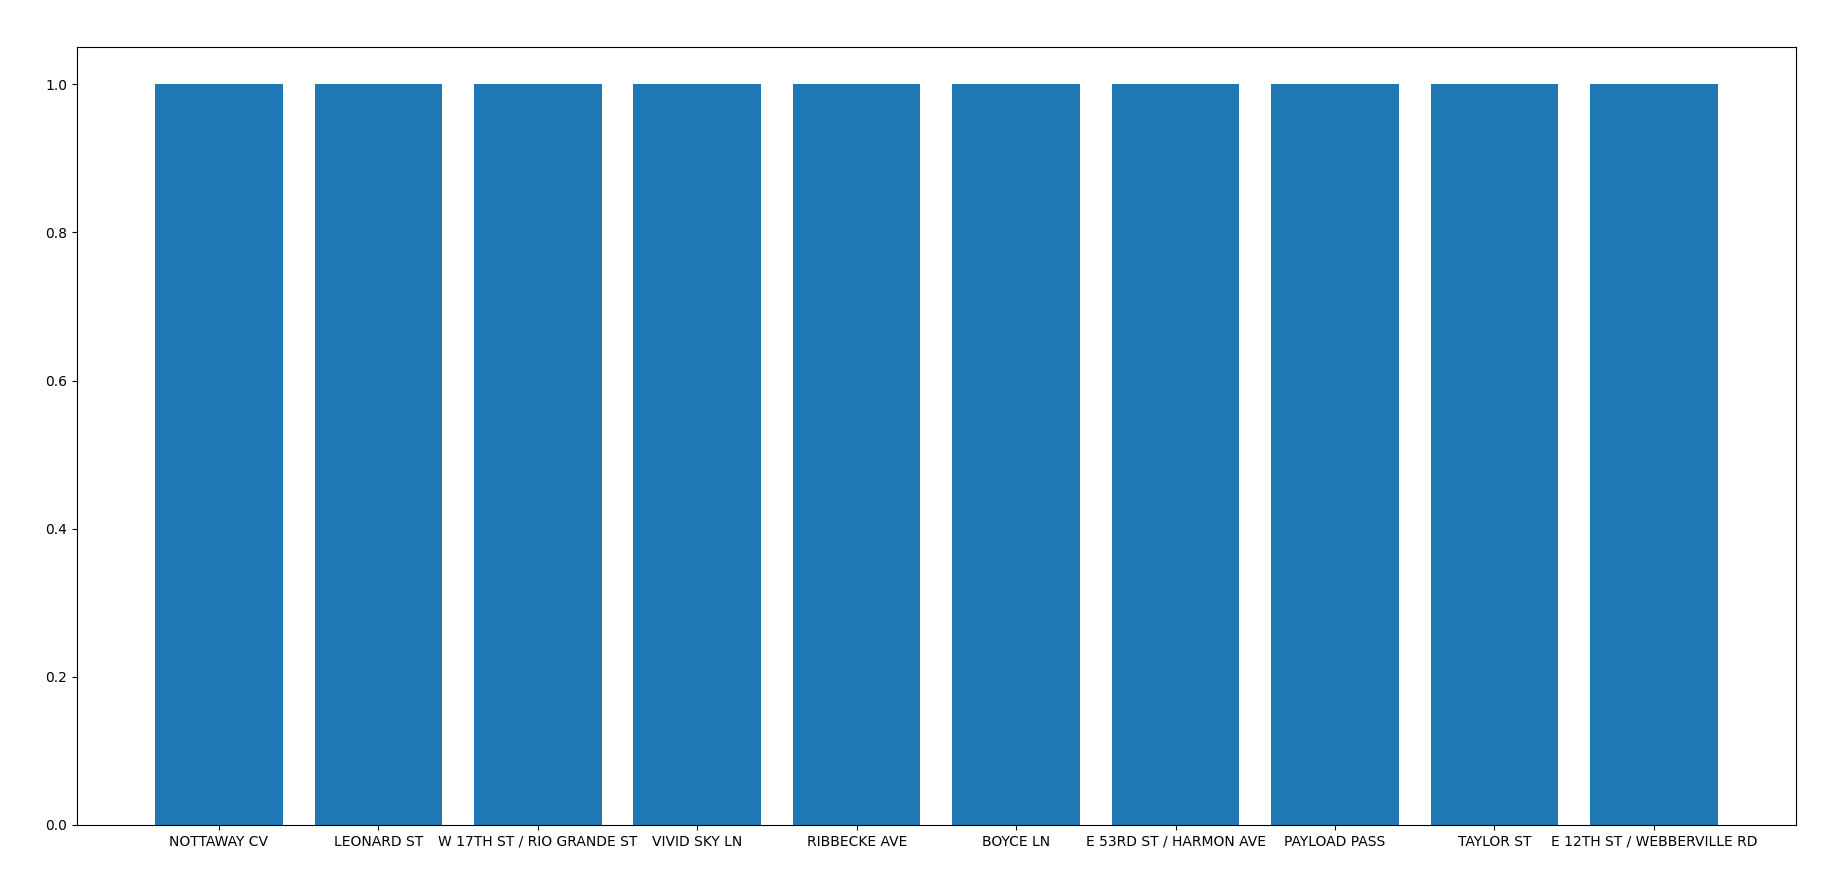
\includegraphics[width=1.6\textwidth]{figures/safest_streets.png}}
  \caption{Ulice s nejnižším počtem zločinů (ulice bez zločinů jsou ignorovány)}
  \label{fig:safest_streets}
\end{figure}

Zákony dodržujícího občana bude zajímat také seřazení čtvrtí podle jejich bezpečnosti. Nejméně bezpečnou
čtvrtí je čtvrť číslo devět. Čtrvť číslo devět je ovšem také centrum města Austin. Nejbezpečnějšími
čtvrtěmi jsou poté čtvrti šest, osm a deset. V případě těchto čtvrtí se zase jedná o odlehlejší a
klidnější čtvrti. \cite{austin-districts}

\begin{figure}
  \centering
  \makebox[\textwidth][c]{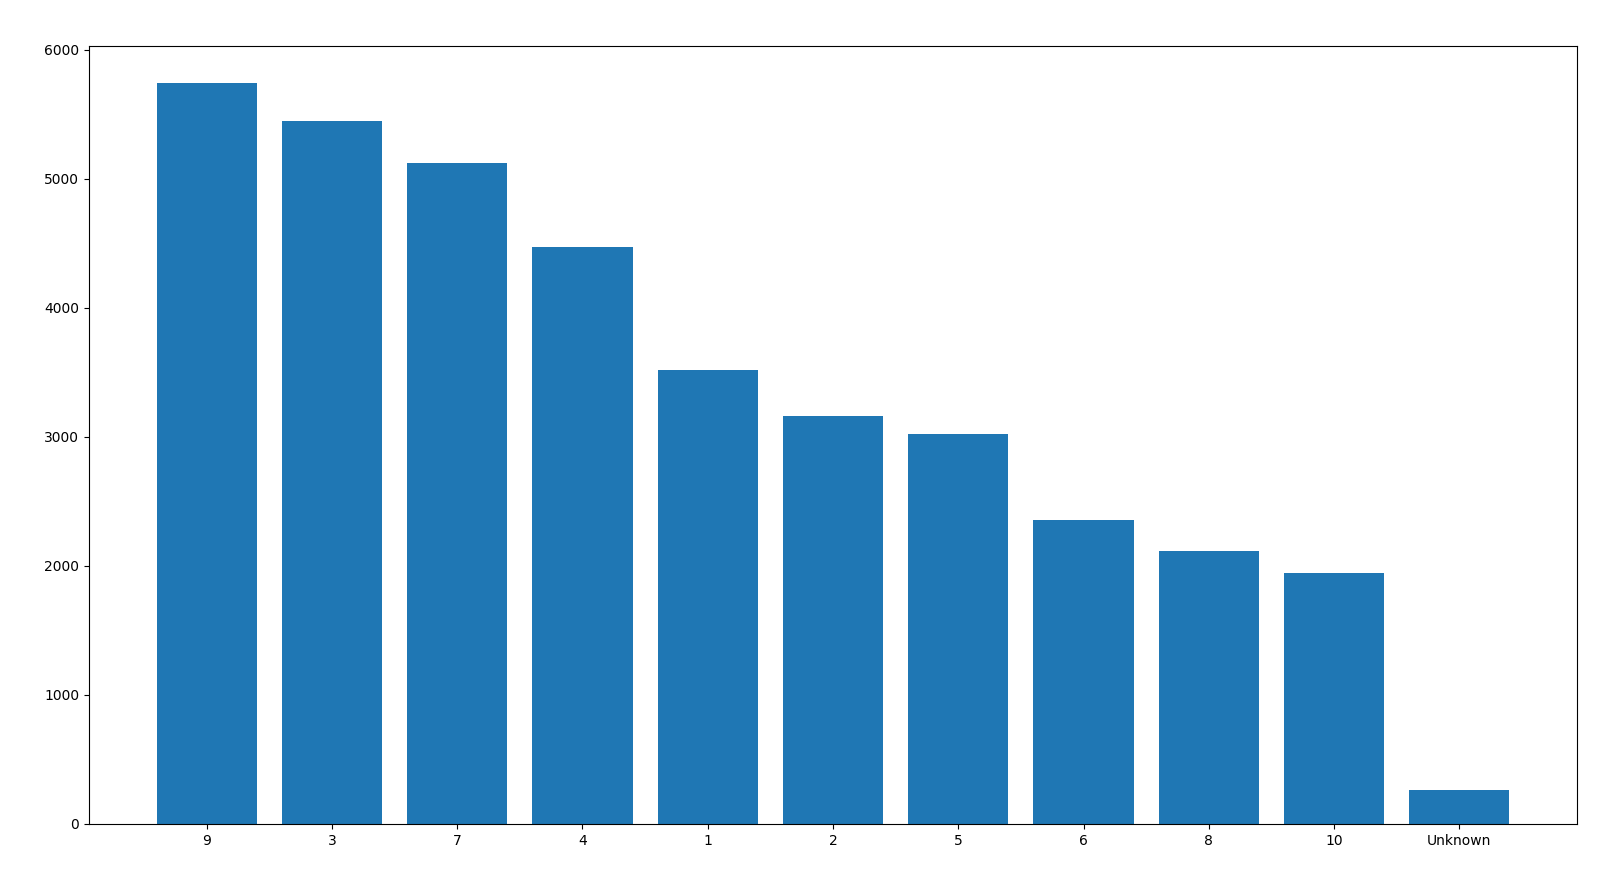
\includegraphics[width=1.6\textwidth]{figures/worst_districts.png}}
  \caption{Čtvrti seřazené podle počtu nahlášených zločinů}
  \label{fig:worst_districts}
\end{figure}

\subsection{Slaughter lane}

Určitou kuriozitou je existence ulice s názvem \emph{Slaughter Lane}. Opět se jedná o relativně dlouhou ulici,
proto nikoho nemůže překvapit vyšší počet nahlášených zločinů. Kuriózní je ovšem fakt, že na východní ani západní
\emph{Slaughter Lane} nebyla nahlášena ani jedna vražda nebo zabití. Lze tedy říct, že se jedná o tzv.
false advertising a ulice \emph{Slaughter Lane} si své jméno nezaslouží.

\begin{figure}
  \centering
  \makebox[\textwidth][c]{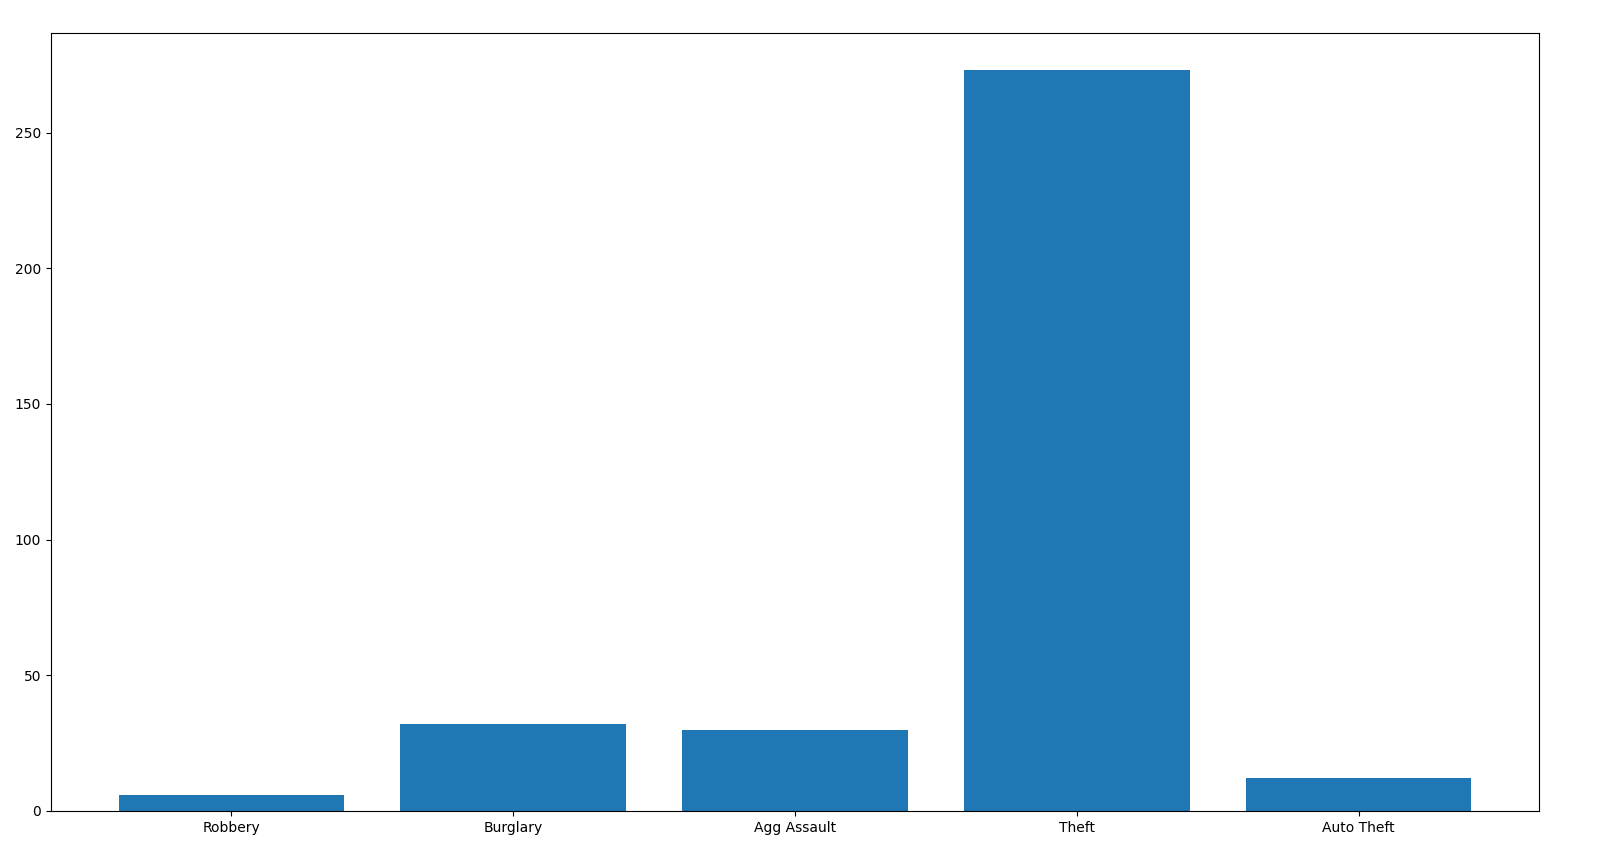
\includegraphics[width=1.6\textwidth]{figures/slaughter_lane.png}}
  \caption{Četnosti zločinů na ulici Slaughter lane}
\end{figure}

\clearpage

\section{Srovnání se zbytkem Spojených států}

Podle oficiálních dat Spojených států \cite{austin-census} žilo v Austinu v roce 2010 asi 790 tisíc obyvatel.
V roce 2020 počet obyvatel vzrostl na přibližně 960 tisíc. Průměrný roční přírůstek tedy byl asi 17 tisíc
nových obyvatel. Pro zjednodušení budeme počítat, že Austin rostl lineárně a v roce 2018 měl Austin 926 tisíc
obyvatel. Přesná data neznáme, neboť se počet obyvatel v průběhu roku měnil, ale také proto, že v daném roce
neproběhlo sčítání obyvatelstva.

Počet obyvatel je důležitý pro relativní srovnání se zbytkem Spojených států. Tabulka \ref{tab:us_crime}
vykazuje statistiku zločinu agregovanou pro celé Spojené státy americké. Tabulka \ref{tab:cities_crime} 
poté vykazuje statistiku agregovanou napříč městy ve Spojených státech. Tato statistika vychází z oficiálních
dat vydaných FBI \cite{us-crime-rates}. A nakonec, tabulka \ref{tab:austin_crime} vykazuje statistiku města 
Austin, tedy data, jež jsou předmětem této analýzy a jež vychází z dat vydaných městem Austin \cite{dataset-source}.

V porovnání s celoamerickou statistikou napříč všemi padesáti státy Austin v~bezpečnosti očividně pokulhává.
Austin má nižší počet napadení a vražd/zabití, v ostatních ohledech ale pokulhává pozadu za průměrem. Tato statistika je
určitým způsobem nepřekvapivá -- celoamerický průměr obsahuje také odlehlé oblasti, menší vesnice, apod.,
tedy místa, kde je zločinnost relativně nízká. V~případě Austinu se naopak jedná o relativně velké město.

Pokud porovnáme město Austin pouze s ostatními americkými městy, statistiky se více srovnají. Austin se vyznačuje
nižším počtem napadení, vražd, přepadení a krádeží vozidel. Počet vloupání je naopak o osminu vyšší než průměr
amerických měst, počet krádeží je o třetinu vyšší než průměr. Alarmující je poté počet znásilnění, který se rovná
skoro dvojnásobku průměru všech měst. Ve prospěch Austinu vypovídá převážně fakt, že počet vražd je oproti průměru o 41 \%
nižší, počet přepadení je poté nižší o 19 \%. Nakonec tak nemůžeme město Austin prohlásit za nadprůměrně bezpečné.
Vyloženě nebezpečné také není, ale relativně vysoký počet znásilnění je alarmující.

\begin{table}
  \centering
  \caption{Celoamerická statistika}
  \label{tab:us_crime}
  \begin{tabular}{ |l|l|l| }
  \hline
      Zločin & Celkový počet & Počet na 100 tisíc obyv. \\
      Znásilnění & 127945 & 44.4 \\
      Vraždy a zabití & 14905 & 5.0 \\
      Přepadení & 265464 & 89.9 \\
      Napadení & 738590 & 250.0 \\ 
      Vloupání & 1097816 & 371.6 \\
      Krádeže vozidla & 692172 & 234.3 \\ 
      Krádeže majetku & 4758121 & 1610.5 \\
  \hline
  \end{tabular}
\end{table}

\begin{table}
  \centering
  \caption{Statistika amerických měst}
  \label{tab:cities_crime}
  \begin{tabular}{ |l|l|l| }
  \hline
      Zločin & Celkový počet & Počet na 100 tisíc obyv. \\
      Znásilnění & 96818 & 48.0 \\
      Vraždy a zabití & 11890 & 5.8 \\
      Přepadení & 236682 & 114.9 \\
      Napadení & 585017 & 283.9 \\ 
      Vloupání & 834355 & 404.9 \\
      Krádeže vozidla & 564989 & 274.2 \\ 
      Krádeže majetku & 3916991 & 1900.8 \\
  \hline
  \end{tabular}
\end{table}

\begin{table}
  \centering
  \caption{Statistika města Austin, TX}
  \label{tab:austin_crime}
  \begin{tabular}{ |l|l|l| }
  \hline
      Zločin & Celkový počet & Počet na 100 tisíc obyv. \\
      Znásilnění & 804 & 86.8 \\
      Vraždy a zabití & 32 & 3.45 \\
      Přepadení & 1022 & 110.37 \\
      Napadení & 2128 & 229.8 \\ 
      Vloupání & 4171 & 450.4 \\
      Krádeže vozidla & 2427 & 262.1 \\ 
      Krádeže majetku & 26572 & 2869.5 \\
  \hline
  \end{tabular}
\end{table}

\clearpage

\begin{thebibliography}{50}

\bibitem{dataset-source}
City of Austin \textit{2018 Annual Crime} [online, cit. 2021-12-28]
Dostupné z: \url{https://data.austintexas.gov/Public-Safety/2018-Annual-Crime/pgvh-cpyq} 
City of Austin, 6. leden 2020

\bibitem{austin-districts}
City of Austin \textit{Council District Map} [online, cit. 2021-12-29]
Dostupné z: \url{https://www.austintexas.gov/GIS/CouncilDistrictMap/} 
City of Austin

\bibitem{austin-census}
United States Census Bureau \textit{U.S. Census Bureau QuickFacts: Austin city, Texas} [online, cit. 2021-12-30]
Dostupné z: \url{https://www.census.gov/quickfacts/fact/table/austincitytexas/LND110210} 
United States Census Bureau

\bibitem{us-crime-rates}
Federal Bureau of Investigation \textit{Council District Map} [online, cit. 2021-12-30]
Dostupné z: \url{https://ucr.fbi.gov/crime-in-the-u.s/2018/crime-in-the-u.s.-2018/tables/table-16} 
Federal Bureau of Investigation

\end{thebibliography}

\end{document}

